\documentclass[useAMS, usenatbib]{mnras}
\pdfsuppresswarningpagegroup=1
%
\usepackage[spanish,es-minimal,english]{babel}
\usepackage[utf8]{inputenc}
\usepackage{graphicx}

\usepackage{xcolor}
\usepackage{hyperref}
\usepackage{siunitx}
\usepackage{newtxtext}
\usepackage[stix2,smallerops]{newtxmath}
\usepackage{booktabs}
\hypersetup{colorlinks=True, linkcolor=blue!50!black, citecolor=black,
  urlcolor=blue!50!black}
\usepackage{etoolbox}
\robustify\bfseries
\robustify\itshape

\usepackage[shortlabels]{enumitem}

\bibliographystyle{mnras}

\sisetup{
  % explicit "+" is useful for velocities
  retain-explicit-plus = true,
  % prefer 10^6 over 1 x 10^6
  retain-unity-mantissa = false,
  % Use x +/- e instead of x(e)  
  separate-uncertainty = true,
  % Make sure to pick up bold font when used in section heading for instance
  detect-weight = true,
}

%% 
%% Will macros
%%
% A better \ion command that works in more circumstances
\newcommand\ION[2]{#1\,\scalebox{0.9}[0.8]{\uppercase{#2}}}
\newcounter{ionstage}
\renewcommand{\ion}[2]{\setcounter{ionstage}{#2}% 
  \ensuremath{\mathrm{#1\,\scriptstyle\Roman{ionstage}}}}
\newcommand\hii{\ion{H}{2}}
\newcommand\nii{[\ion{N}{2}]}
\newcommand\oiii{[\ion{O}{3}]}
\newcommand\oii{[\ion{O}{2}]}
\newcommand\Wav[1]{\ensuremath{\lambda #1}}

\title[HH 529 II and III in the Orion Nebula]{
  Photoionized Herbig-Haro objects in the Orion Nebula I: HH 529 II and III
}

\author[J. E. M\'endez-Delgado et al.]
{J. E. M\'endez-Delgado$^{1,2}$ \thanks{E-mail: jemd@iac.es},
  C. Esteban$^{1,2}$, J. Garc{\'{\i}}a-Rojas$^{1,2}$, W. J. Henney$^{3}$  
  \newauthor 
  and K. Z. Arellano-C\'ordova$^{1}$ and collaborators\\
\\
% List of institutions
$^{1}$Instituto de Astrof\'isica de Canarias (IAC), E-38205 La Laguna, Spain\\
$^{2}$Departamento de Astrof\'isica, Universidad de La Laguna, E-38206 La Laguna, Spain\\
$^{3}$Instituto de Radioastronom\'ia y Astrof\'isica, Universidad Nacional Aut\'onoma de M\'exico, Apartado Postal 3-72, 58090 Morelia, Michoac\'an, M\'exico}


\begin{document}

\section{Proper motions of HH~529 II and III}
\label{sec:proper-motions-hh}
% ODell:2015a gives III: V_t = 7 km/s and V_r = -28 kn/s (helio), so -54 wrt OMC
% ODell:2008a gives III: V_t = 41 km/s and V_r = -30 km/s
% ODell:2008a gives II: V_t = 92 km/s and V_r = -31 km/s

\begin{table}
  \caption{Proper motions of shock features}
  \label{tab:proper-motions}
  \begin{tabular}{@{}lcSSS@{}}
    \toprule
     & UVES & {\(V_\text{t}\)} & {PA} & {Contrast}\\
    Feature & cut & {\si{km.s^{-1}}} & {deg} & {\(S(\mathrm{H\alpha}) / S(\mathrm{H\alpha,BG})\)} \\
    \midrule
    {(1)} & {(2)} & {(3)} & {(4)} & {(5)}  \\
    \addlinespace 
    HH 529 III a1 & & 33 \pm 3 & 90  \pm  3 & 0.46 \pm 0.14\\
    HH 529 III a2 &3& 36 \pm 1 & 107 \pm 7 & 0.82 \pm 0.11\\
    HH 529 III a3 & & 32 \pm 1 & 117  \pm  3 & 0.52 \pm 0.14\\
    HH 529 III a4 & & 39 \pm 2 & 137  \pm  5 & 0.41 \pm 0.07\\
    HH 529 III a5 & & 32 \pm 1 & 152  \pm 10 & 0.27 \pm 0.07\\
    \addlinespace   
    HH 529 III b1 &3& 30 \pm 2 & 105  \pm 3 & 0.95 \pm 0.09\\
    HH 529 III b2 & & 27 \pm 1 & 130  \pm 1 & 1.14 \pm 0.10\\
    HH 529 III b3 & & 30 \pm 2 & 125  \pm 4 & 0.64 \pm 0.07\\
    \addlinespace
    HH 529 II a &2& 21 \pm 9 & 117  \pm 58 & 0.25 \pm 0.03\\
    HH 529 II b &2& 26 \pm 5 & 107  \pm  4 & 0.35 \pm 0.08\\
    HH 529 II c & & 35 \pm 9 & 151  \pm 87 & 0.22 \pm 0.03\\
    \bottomrule
    \addlinespace
    \multicolumn{5}{@{}p{\linewidth}@{}}{
    \textsc{Columns:}
    (1)~Name of shock feature (see Fig.~\ref{fig:proper-motions} for positions).
    (2)~Spatial cut of the UVES spectrum where this feature appears, if any.
    (3)~Mean tangential velocity for each feature,
    weighted by background-subtracted surface brightness,
    \(S(\mathrm{H\alpha})\), of each pixel.
    (4)~Mean position angle of proper motion,
    weighted in the same way.
    (5)~Mean relative H\(\alpha\) brightness with respect to nebular background.
    For columns 3, 4, and 5, the \(\pm\) uncertainties correspond to the
    root-mean-square variation over each sample region and do not include systematic uncertainties,
    which are of order \SI{2}{km.s^{-1}}
    }
\end{tabular}
\end{table}

\begin{figure}
  \centering
  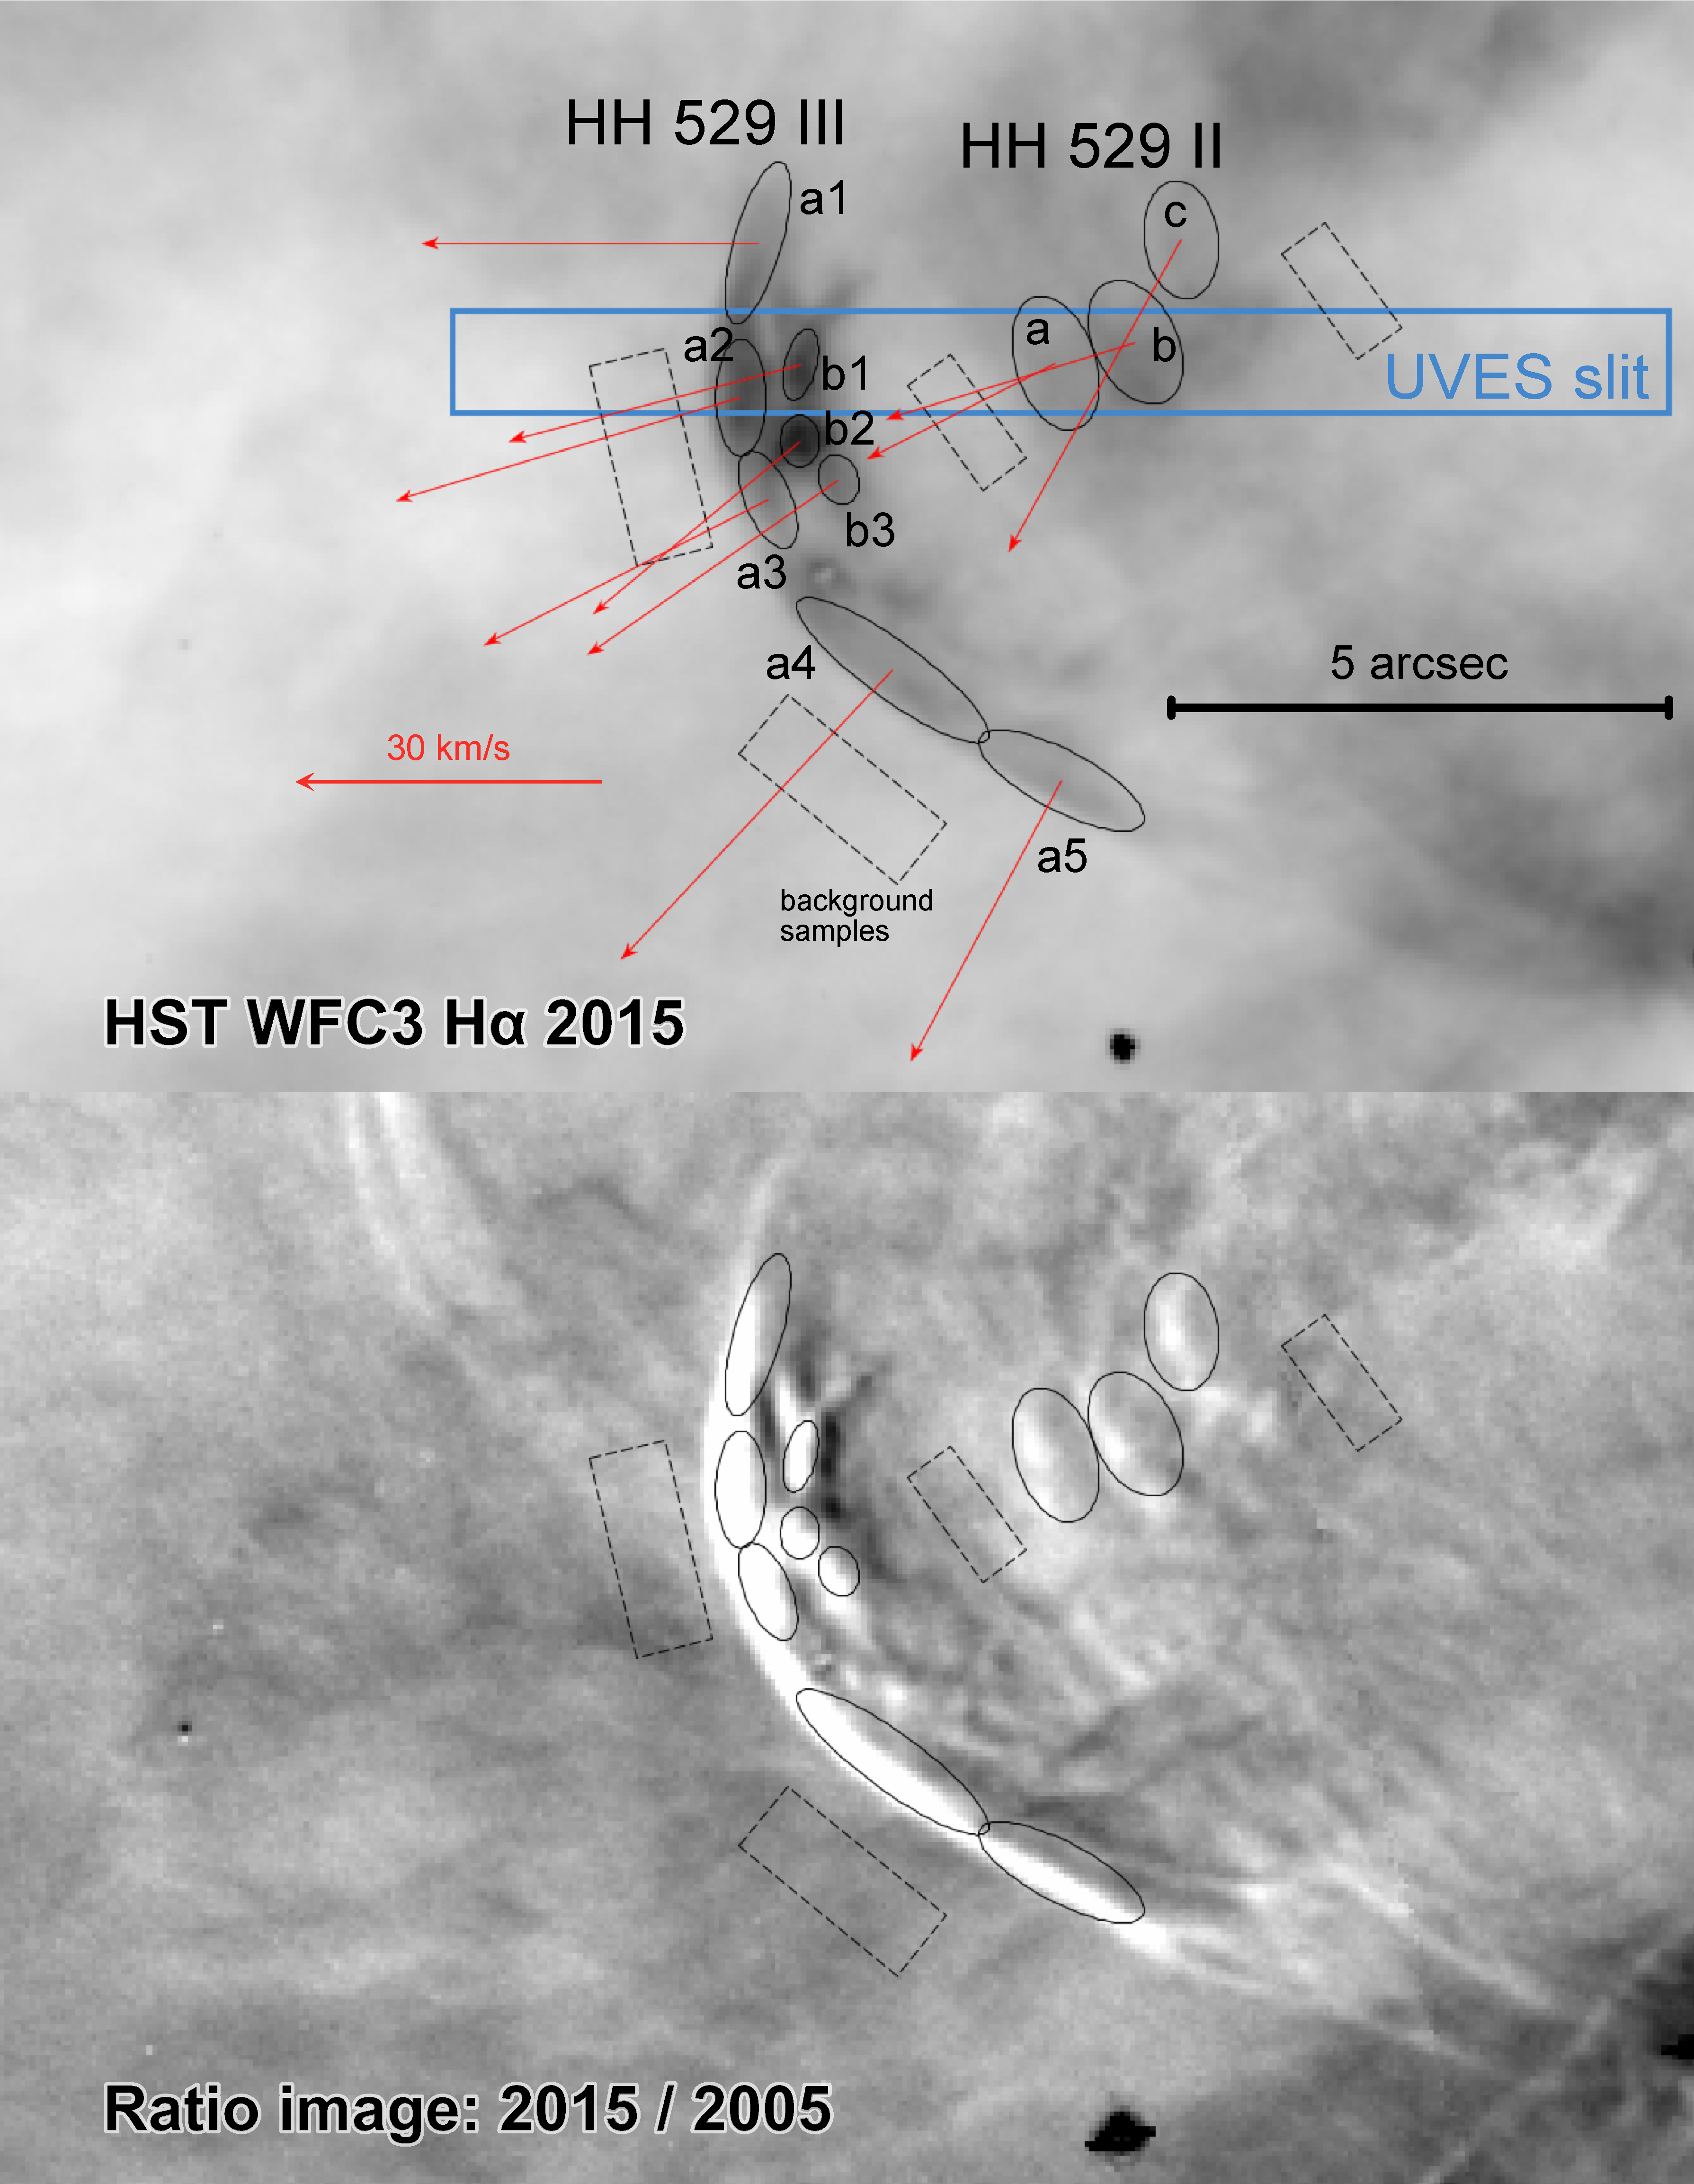
\includegraphics[width=\linewidth]{hh529-halpha-proper-motions-annotated}
  \caption{
    Tangential velocities of shock features in HH~529~II and III
    derived from 3 epochs of HST imaging.
    Upper panel shows various discrete features identified in the bow shocks
    (black ellipses with arrows indicating the average proper motion of each feature).
    Small dashed rectangles indicate regions where the nebular background brightness was measured
    and the large blue rectangle shows the position of the spectrograph slit.
    The backgound negative grayscale shows an \textit{HST} WFC3 image in the F656N filter from 2015.
    Lower panel shows the ratio between the 2015 image and an \textit{HST} ACS image
    in the F658N filter from 2005 (white means brighter in 2015).
    This highlights the changes in the nebula over that 10-year period,
    which are principally due to motions of the shocked gas.
  }
  \label{fig:proper-motions}
\end{figure}

\begin{table}
  \caption{HST observations used in proper motion study}
  \label{tab:programs}
  \setlength\tabcolsep{1ex}
  \begin{tabular}{llll}
    \toprule
    Date & Program & Camera, CCD, Filter & Reference \\
    \midrule
    1995-03 & 5469 & WFPC2, PC, F656N & \citet{Bally:1998a} \\
    2005-04 & 10246 & ACS, WFC, F658N & \citet{Robberto:2013a} \\
    2015-01 & 13419 & WFC3, UVIS, F656N & \citet{Bally:2018c} \\
    \bottomrule
  \end{tabular}
\end{table}


The plane-of-sky motions of the bow shocks in HH~529 have been previously reported
in Table~3 of \citet{ODell:2008a} and in sec~3.3.1.3 of \citet{ODell:2015a}.
However the reported tangential velocities are very disparate,
so we have re-measured the proper motions,
taking advantage of the 20~years of archival
\textit{Hubble Space Telescope} (\textit{HST}) imaging that is now available.
Results are presented in Table~\ref{tab:proper-motions} and Figure~\ref{fig:proper-motions}.

We employ three epochs of observations, as detailed in Table~\ref{tab:programs}.
All data was downloaded from the Barbara~A. Mikulski Archive for Space Telescopes%
\footnote{MAST, \url{https://archive.stsci.edu/}}
and the 1995 and 2015 images were aligned to the 2005 ACS image using Astrodrizzle%
\footnote{\url{https://drizzlepac.readthedocs.io}}
and rebinned to the ACS pixel scale of \SI{0.05}{arcsec}.
The 2005 image itself has been aligned to the absolute astrometric reference of 2MASS,
as painstakingly described in sec~3.3 of \citet{Robberto:2013a}.
Proper motions are estimated for the two intervals, 1995--2005 and 2005--2015,
using the Fourier Local Correlation Tracking (FLCT) method
\citep{Welsch:2004a, Fisher:2008a}\footnote{
  We used version 1.07 of FLCT, obtained from \url{http://cgem.ssl.berkeley.edu/cgi-bin/cgem/FLCT/home},
  together with version 1.04 of the Python wrapper pyflct,
  obtained from \url{https://github.com/PyDL/pyflct}.}
with a kernel width of 10~pixels (\SI{0.5}{arcsec}).
For an assumed distance of \SI{417}{pc},
a shift of 1~pixel in 10~years corresponds to approximately \SI{10}{km.s^{-1}}.
A potential disadvantage of using the ACS data in this study
is that the F658N ACS filter is relatively broad and includes both
H\(\alpha\) \Wav{6563} and \nii{} \Wav{658\includegraphics[width=\linewidth]{will-529-III-motions.tex}3},
whereas the WFPC2 and WFC3 F656N filters are narrower and more effectively isolate \Wav{6563}.
Ionization gradients in the nebula can therefore contribute to differences in the images obtained,
which would obscure the signal due to the gas motions.
However, the degree of ionization in HH~529~III and II is so high that this turns out not to be an issue in this object.

We find that HH~529~III consists of at least two distinct moving structures.
The large outer curved bow, which we call III~a, is relatively smooth,
spanning about \SI{7}{arcsec} in its brightest part,
but with fainter wings (best visible on the ratio image) that extend farther.
We cover the bright part of the bow with 5 sample ellipses: a1 to a5,
where a3 seems to be the apex of the bow but a2 is the one that falls in the UVES slit.
Roughly \SI{0.7}{arcsec} to the east of III~a is a smaller, knottier bow, which we call III~b and cover with 3 sample ellipses: b1, b2 and b3.
The brightest knot is b2, but it is the b1 sample that falls in the UVES slit.
HH~529~II is found to consist of three distinct bows with separations of order \SI{1}{arcsec}, which we call II~a, II~b, and II~c, with II~a and II~b falling in the UVES slit. 


\bibliography{will-529-III-refs}

\end{document}
%%% Local Variables:
%%% mode: latex
%%% TeX-master: t
%%% End:
